\documentclass[12pt]{article}
\usepackage{amsmath,amssymb,amsthm}
\usepackage[english]{babel}
\usepackage[utf8]{inputenc}
\usepackage{fancyhdr}
\usepackage{changepage} 

% for line spacing
\usepackage{setspace}

% for absolute value
\usepackage{commath}

% for numbering
\usepackage{enumerate}

% for image placing
\usepackage{float}

% paper size and margins
\usepackage[letterpaper, left=20mm, right=20mm, top=25mm, bottom = 25mm, headsep=.15in]{geometry}

% for curly brace
\usepackage{amsmath}

% for input images
\usepackage{graphicx}
\graphicspath{ {./} }
\usepackage{subfig}

% for printing pseudocode
\usepackage[boxed]{algorithm}
\usepackage[noend]{algpseudocode}

% for tables
\usepackage{tabularx}

\makeatletter
\def\BState{\State\hskip-\ALG@thistlm}
\makeatother

% for circled numbers
\usepackage{tikz}
\newcommand*\circled[1]{\tikz[baseline=(char.base)]{
            \node[shape=circle,draw,inner sep=1pt] (char) {#1};}}

% double line space
\renewcommand{\baselinestretch}{2.0}

% header, footer and page number
\pagestyle{fancy}
\fancyhf{}
\rhead{Tiankai Jiang \quad 20834939}
\lhead{ECE657A \quad Assignment 2}
\fancyfoot[C]{\thepage}

\setlength{\headheight}{15pt}

\begin{document}
\noindent
\textbf{\large Question 1:}\\
\textbf{Normalization}
\begin{center}
    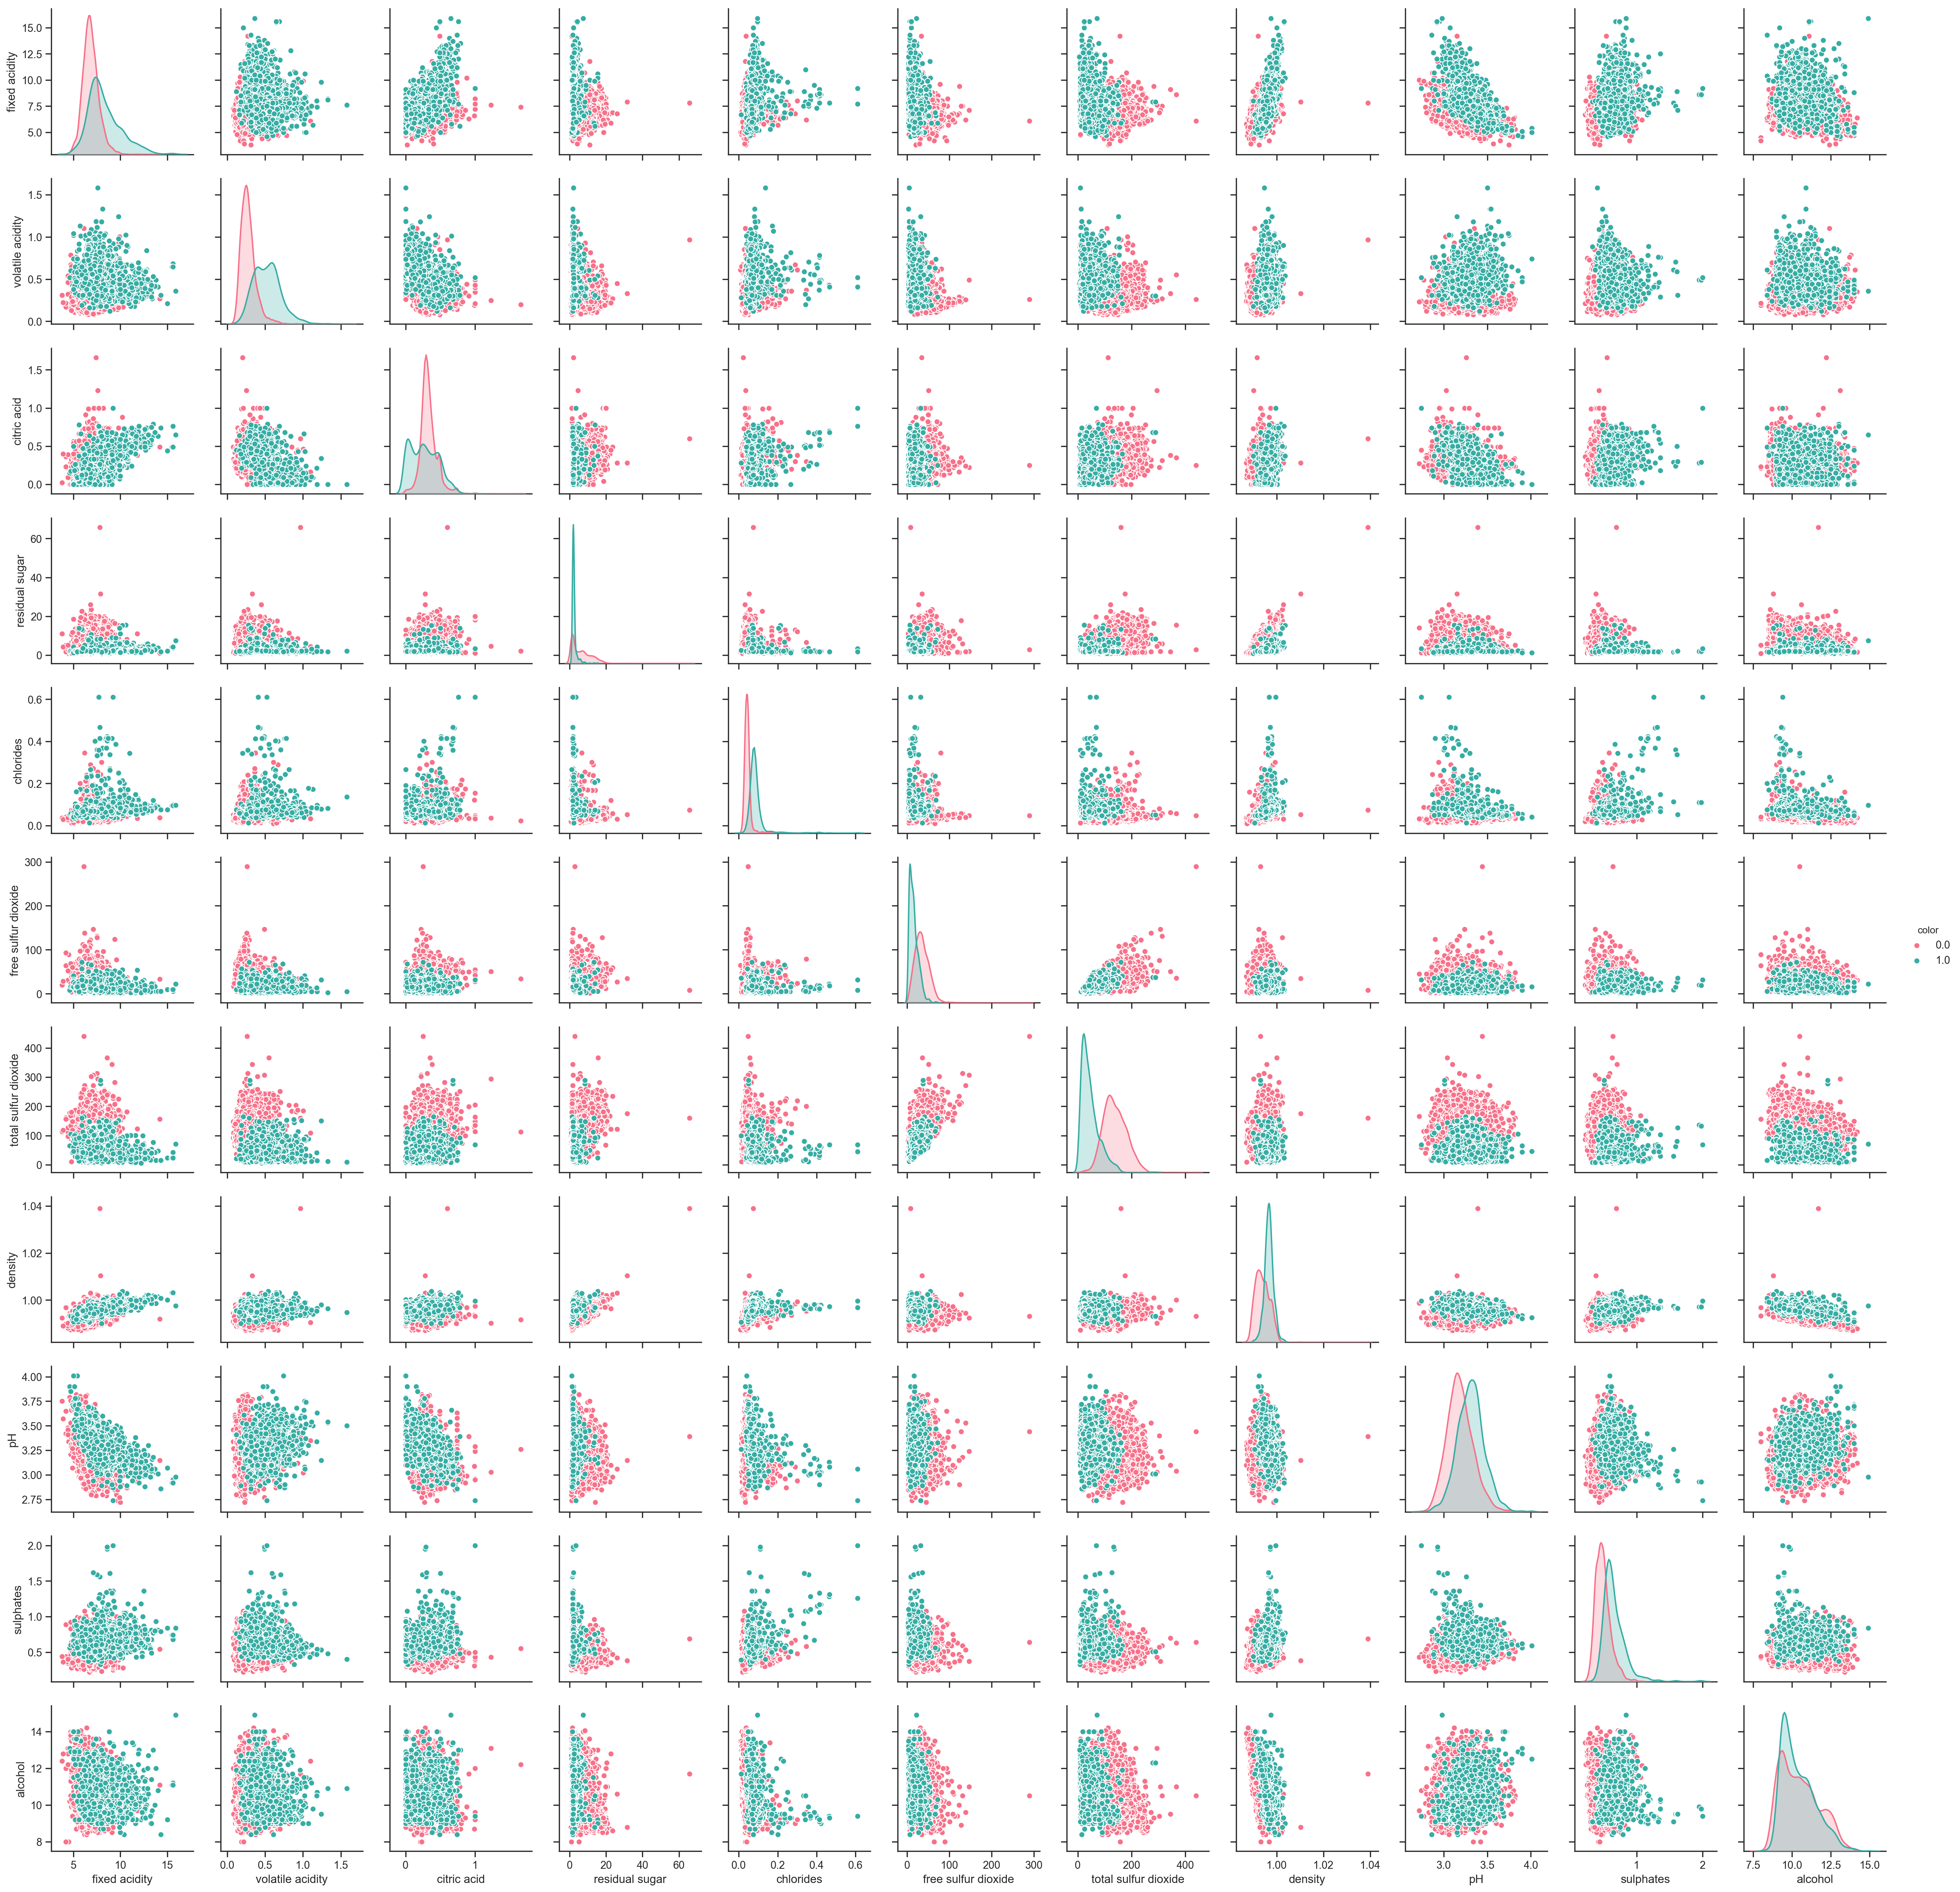
\includegraphics[width=17cm]{Q1_no_normalization.png}
    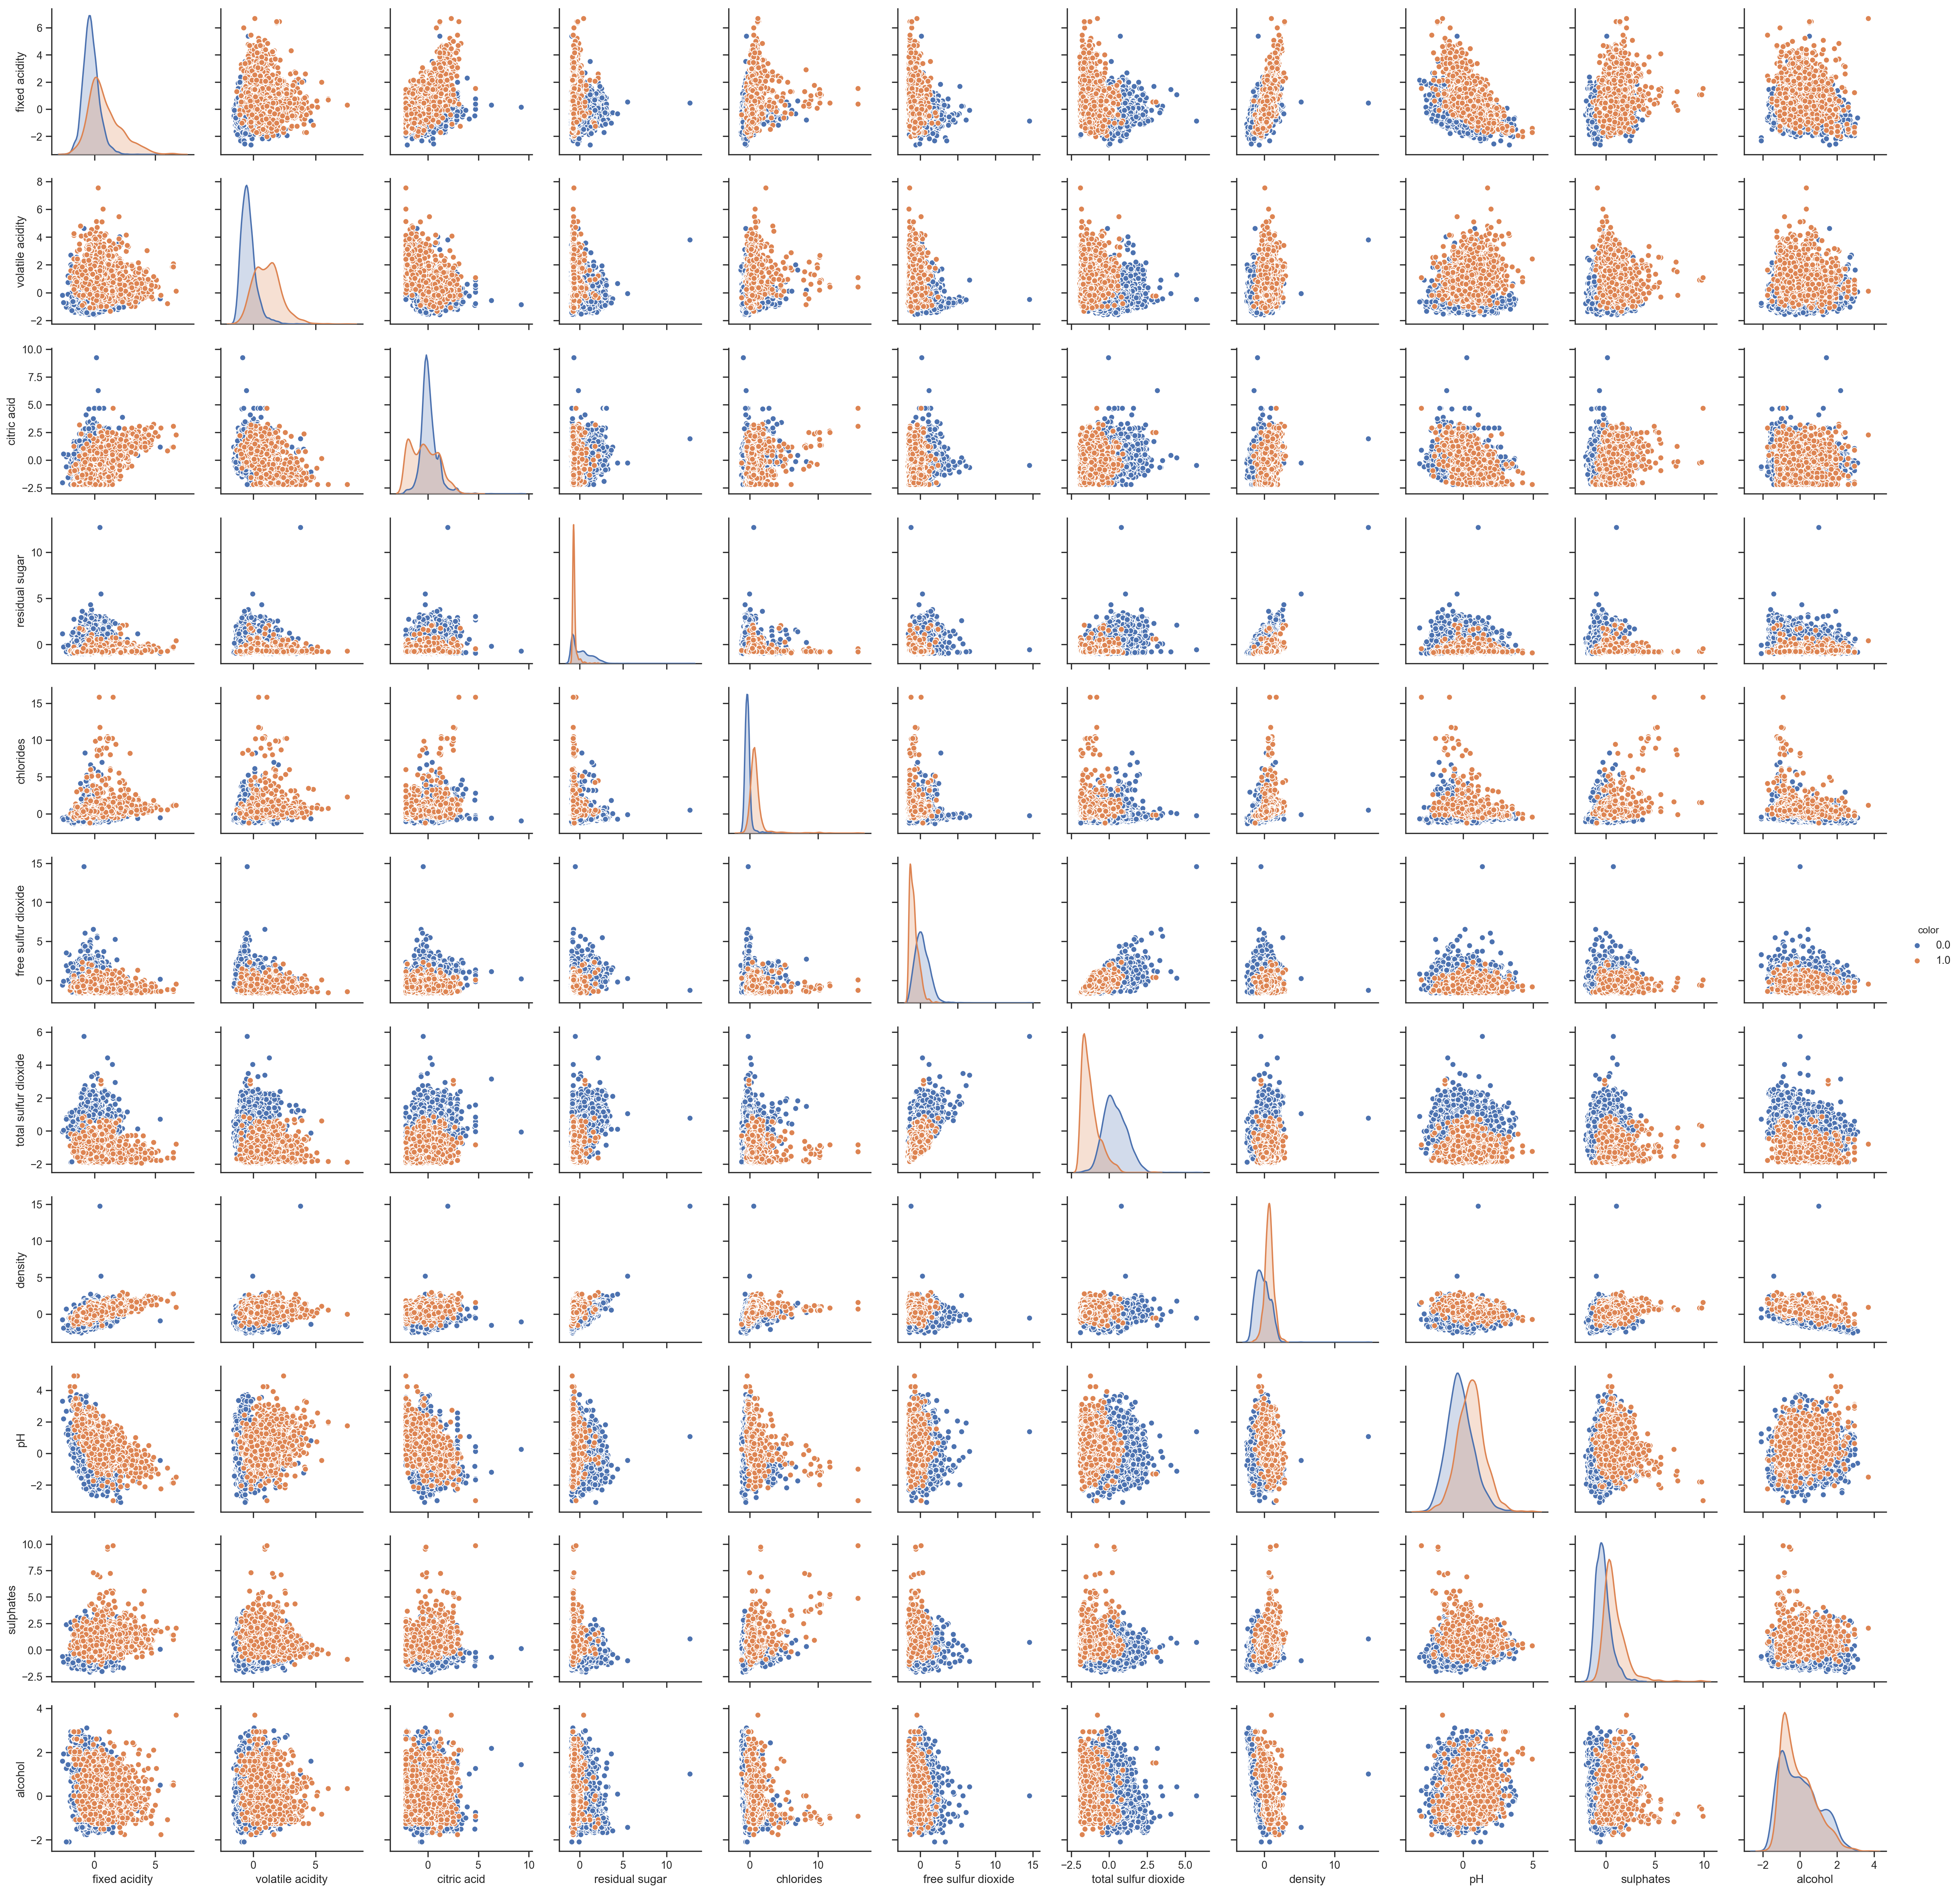
\includegraphics[width=17cm]{Q1_zscore_normalization.png}
\end{center}
\noindent
The first graph is plotted without normalization and the second is plotted after z-score normalization. Points in both plots have the same distribution. However, the range of the axes of the unnormalized plot varies with each feature, but that of the normalized plot are all the same -- the majority of points scattered between -2 to 5 on both axes, with a mean of zero.\\\\
\textbf{KNN Classification With All Features}
\begin{figure}[H]
\captionsetup[subfigure]{labelformat=empty}
\centering
\subfloat[]{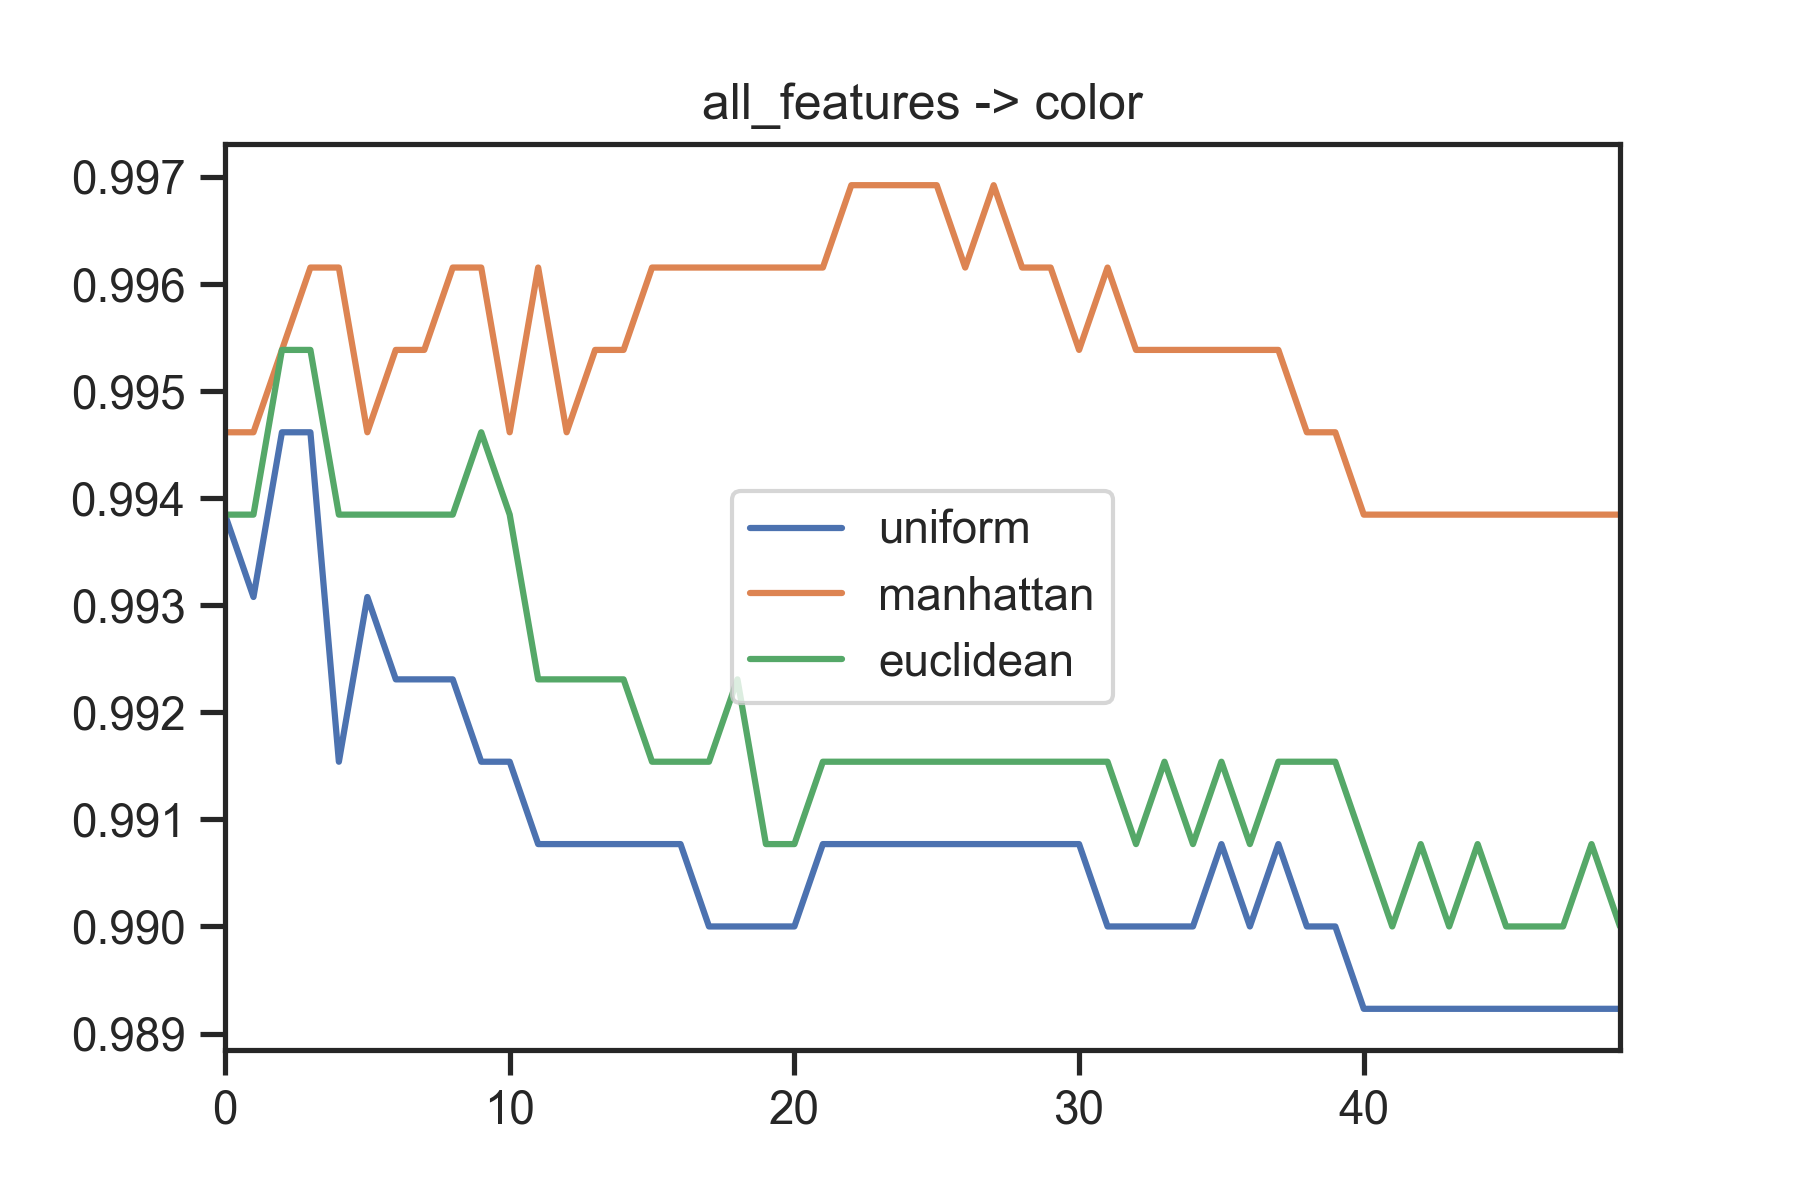
\includegraphics[width=0.48\textwidth]{Q1_all_features_color}}
\subfloat[] {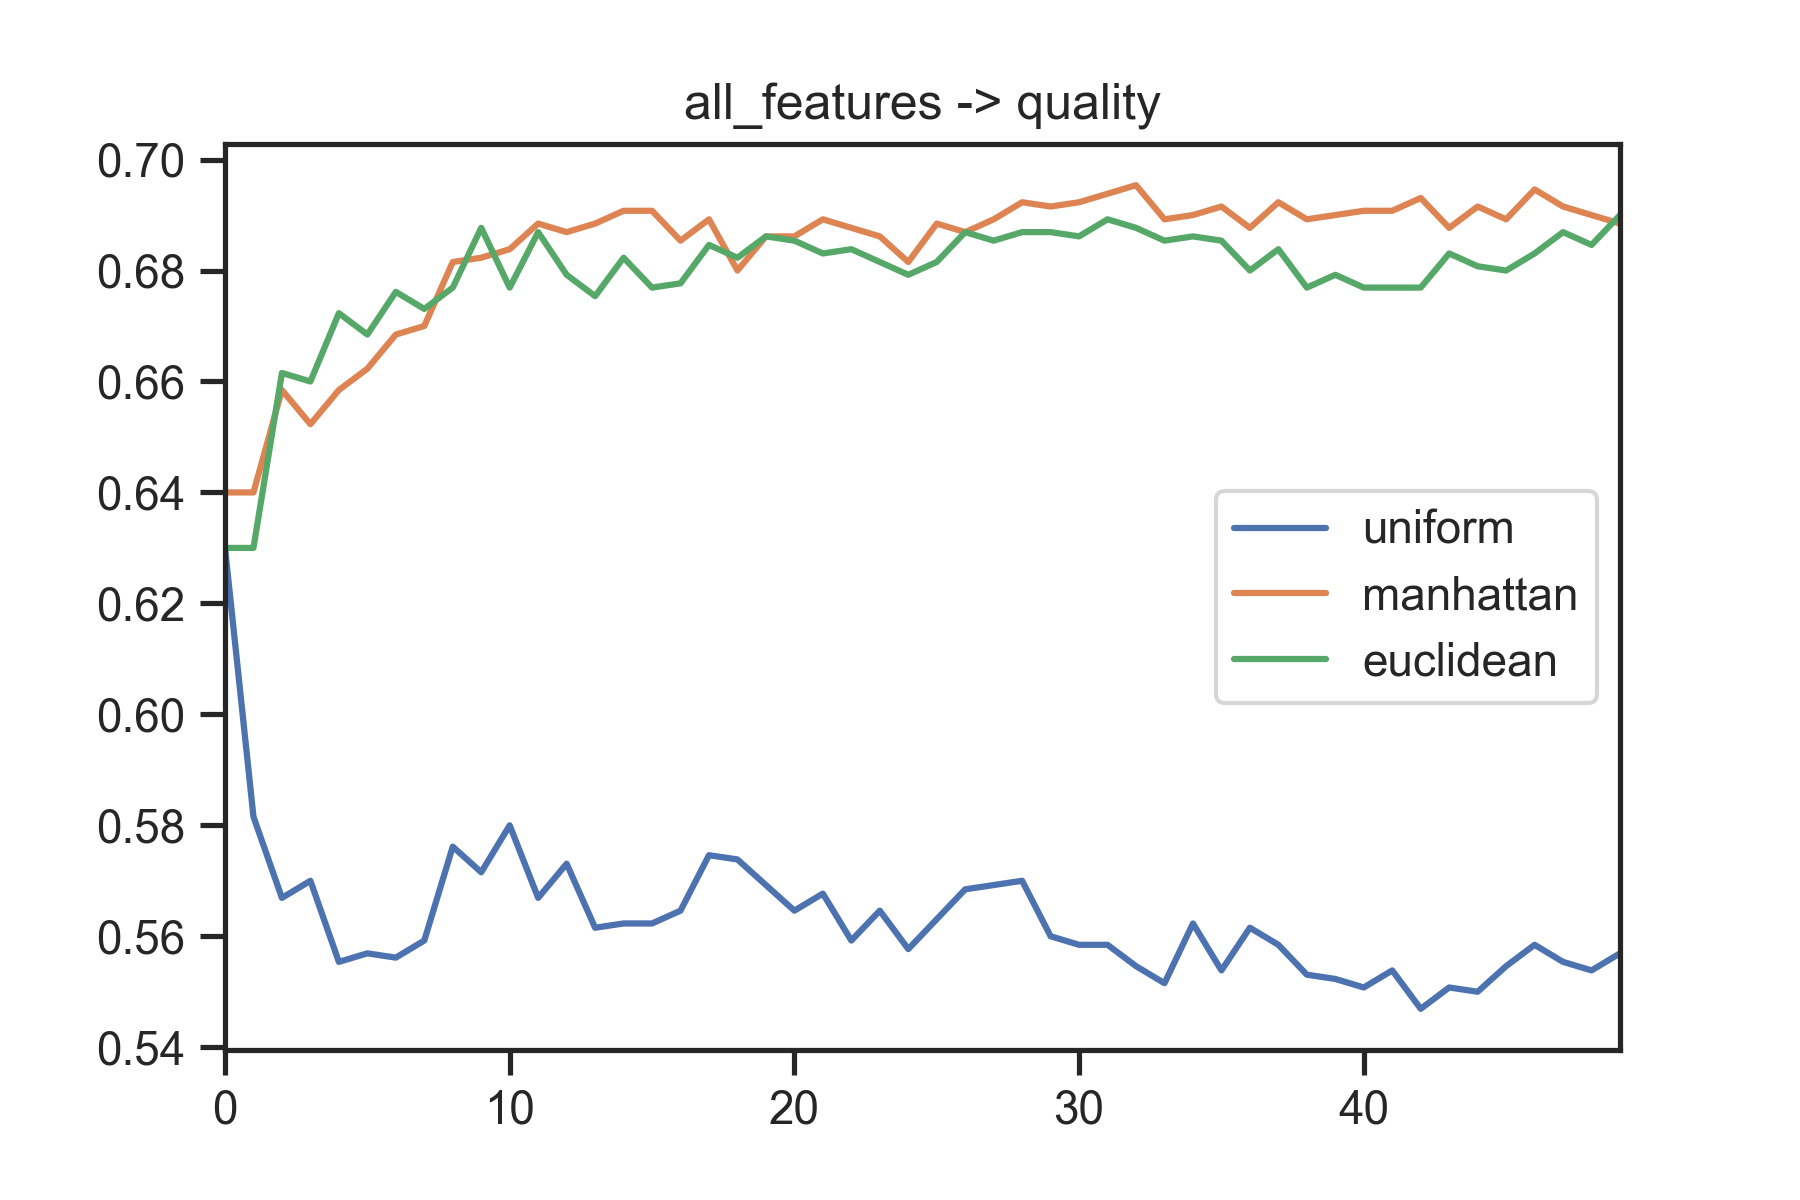
\includegraphics[width=0.48\textwidth]{Q1_all_features_quality.png}}
\end{figure}
\vspace*{-1.5cm}
\noindent
\textbf{KNN Classification With Selected 4 Features}\\
Try all ${11 \choose 4}$ feature combinations and choose the best result.\\
For color prediction under manhattan, no combination of 4 is better than using all features.\\
For color prediction under euclidean, using 'residual sugar', 'total sulfur dioxide', 'density', 'alcohol' yields the best result.
\begin{center}
    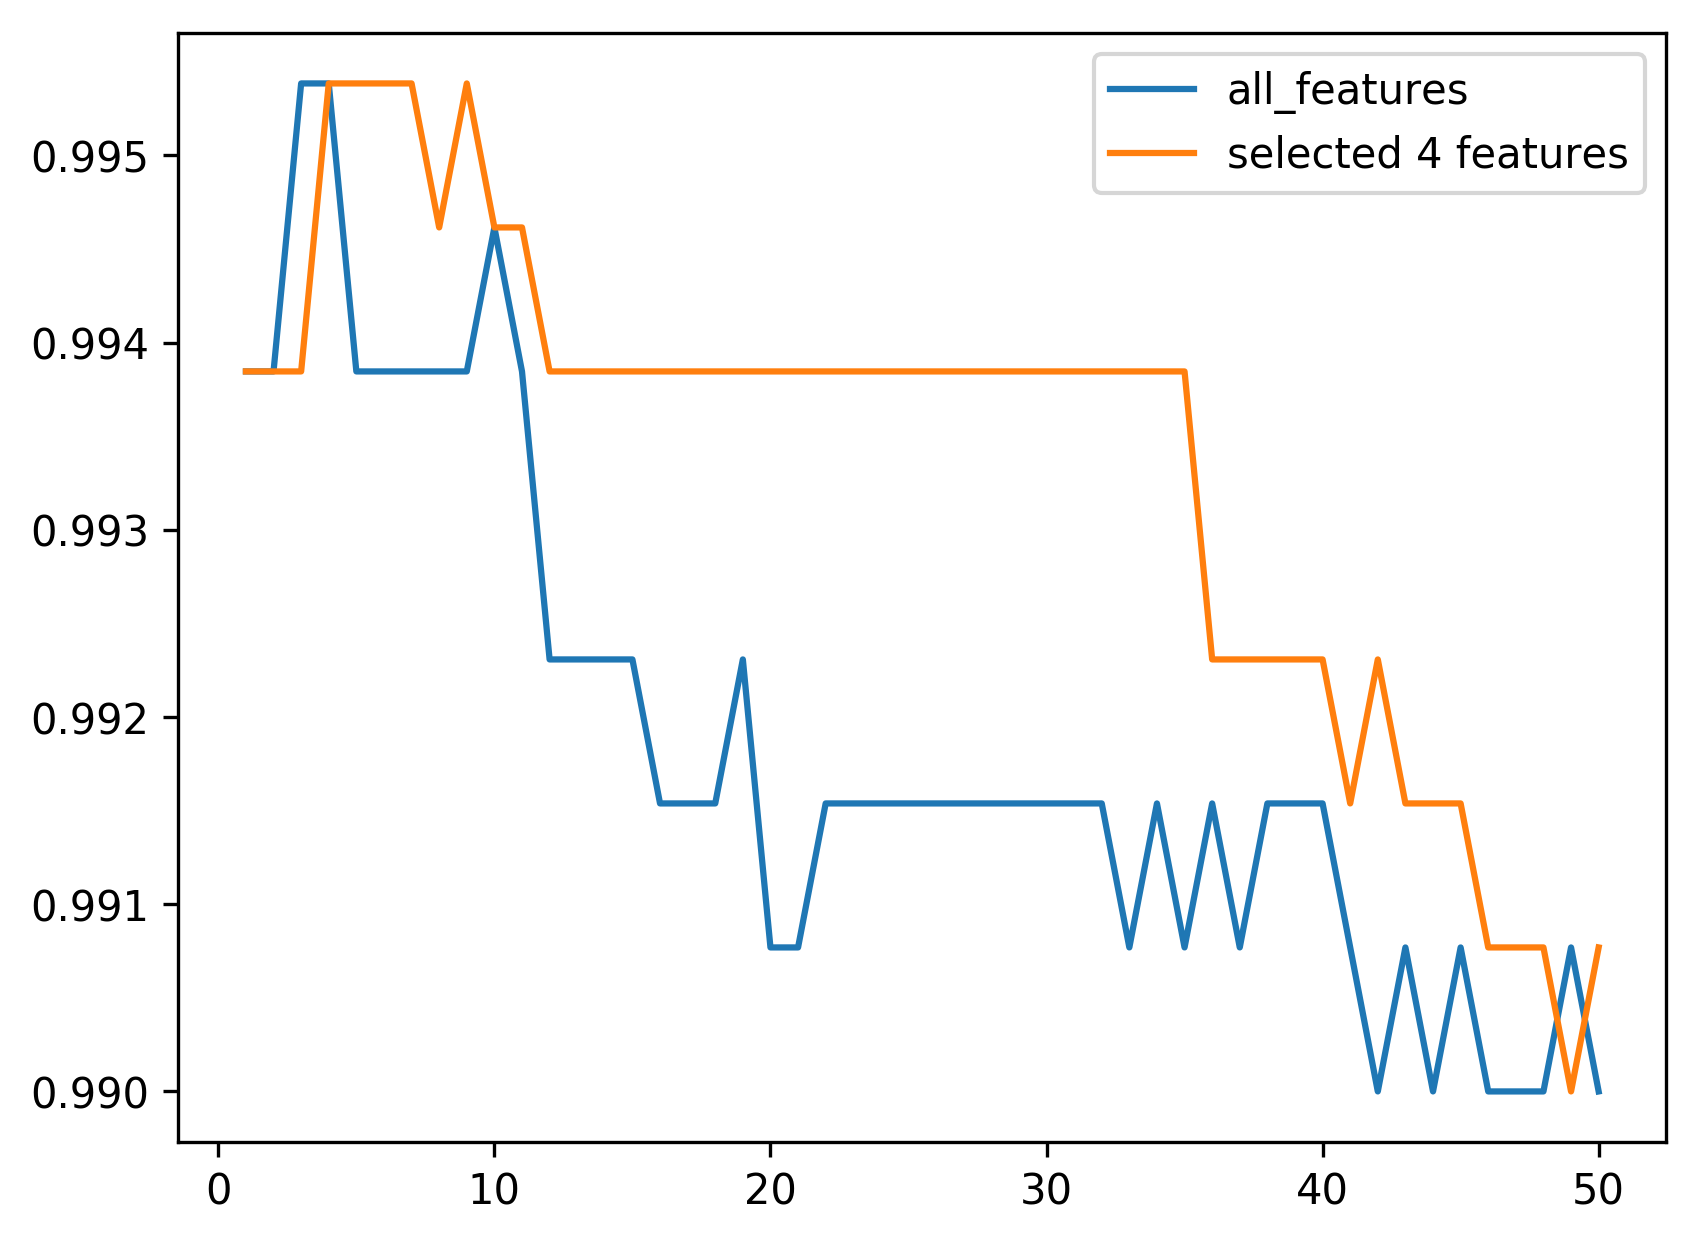
\includegraphics[width=9cm]{./select4features/color_e.png}
\end{center}
\noindent
For color prediction under uniform, using 'residual sugar', 'chlorides', 'total sulfur dioxide', 'density' yields the best result.
\begin{center}
    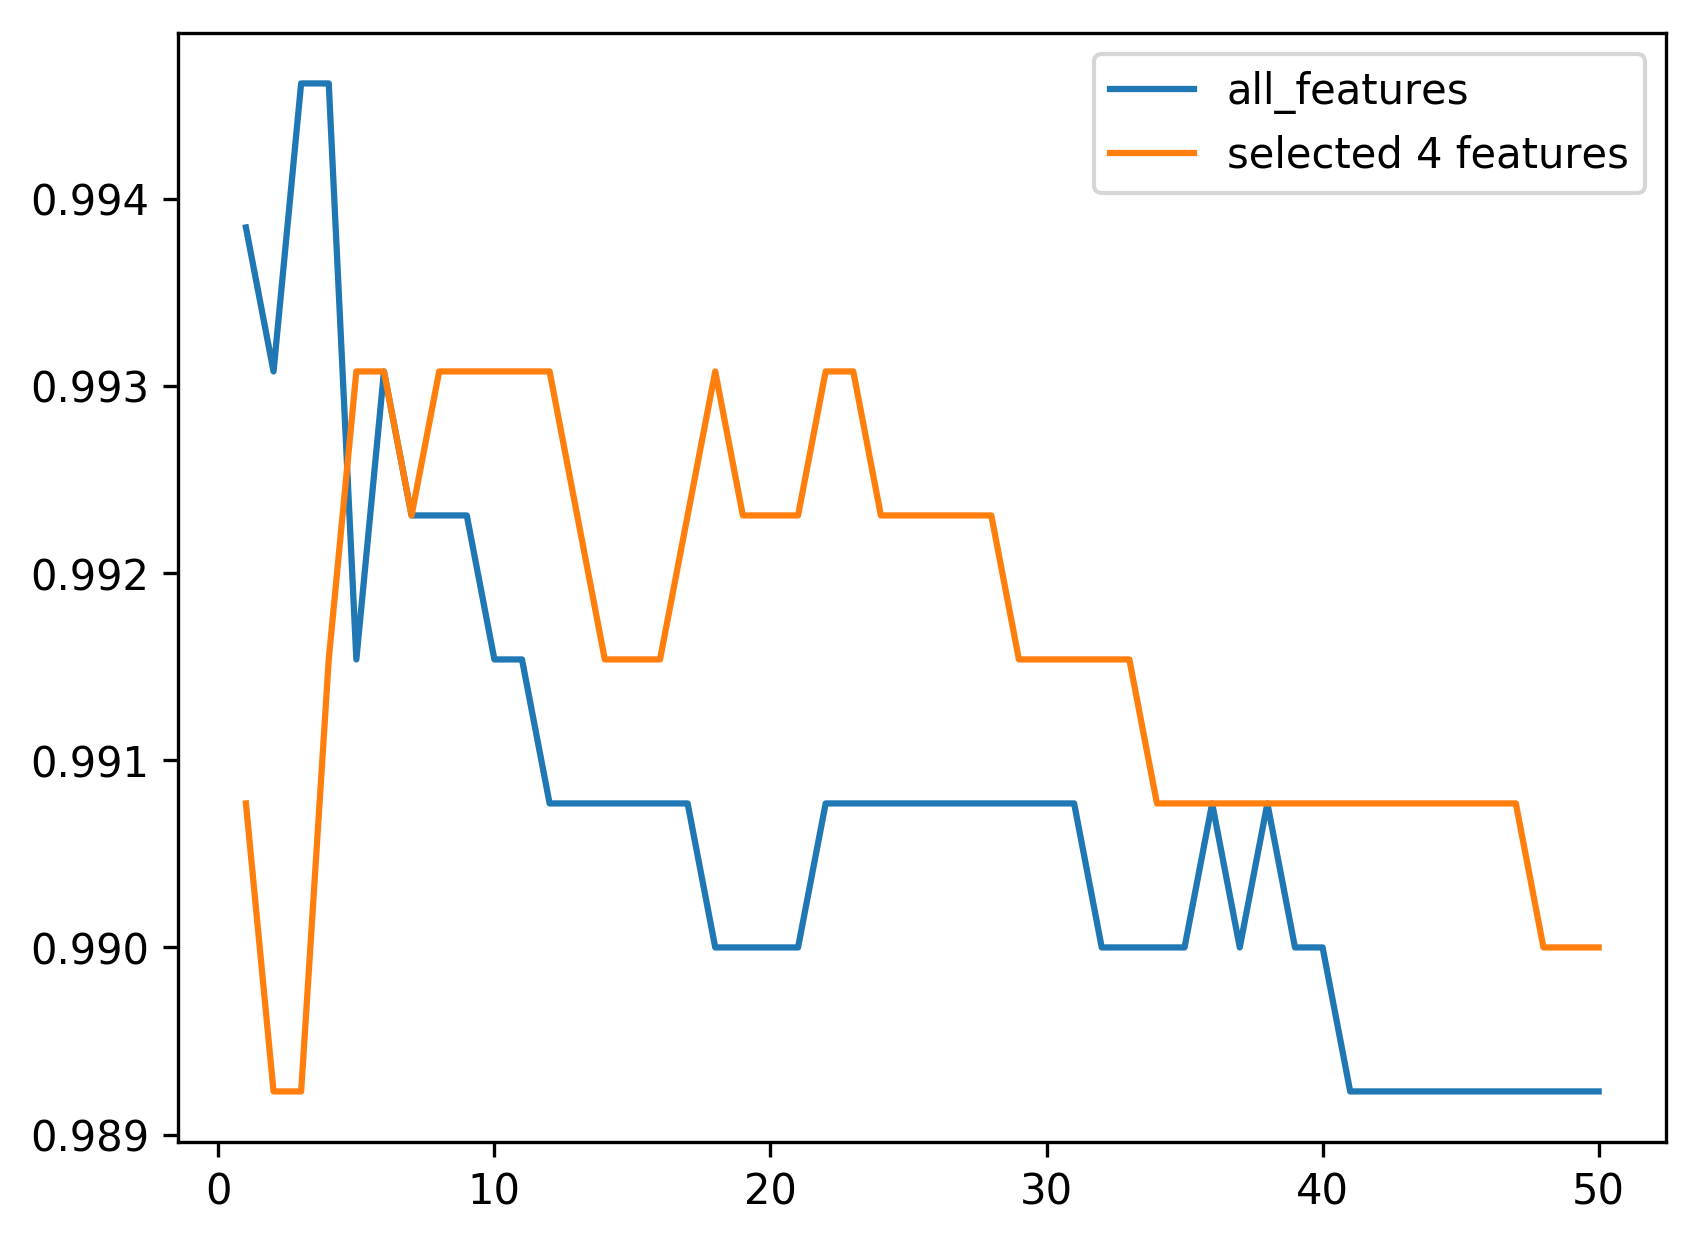
\includegraphics[width=9cm]{./select4features/color_u.png}
\end{center}
\noindent
For quality prediction under manhattan, no combination of 4 is better than using all features.\\
For quality prediction under euclidean, using 'volatile acidity', 'total sulfur dioxide', 'sulphates', 'alcohol' yields the best result.
\begin{center}
    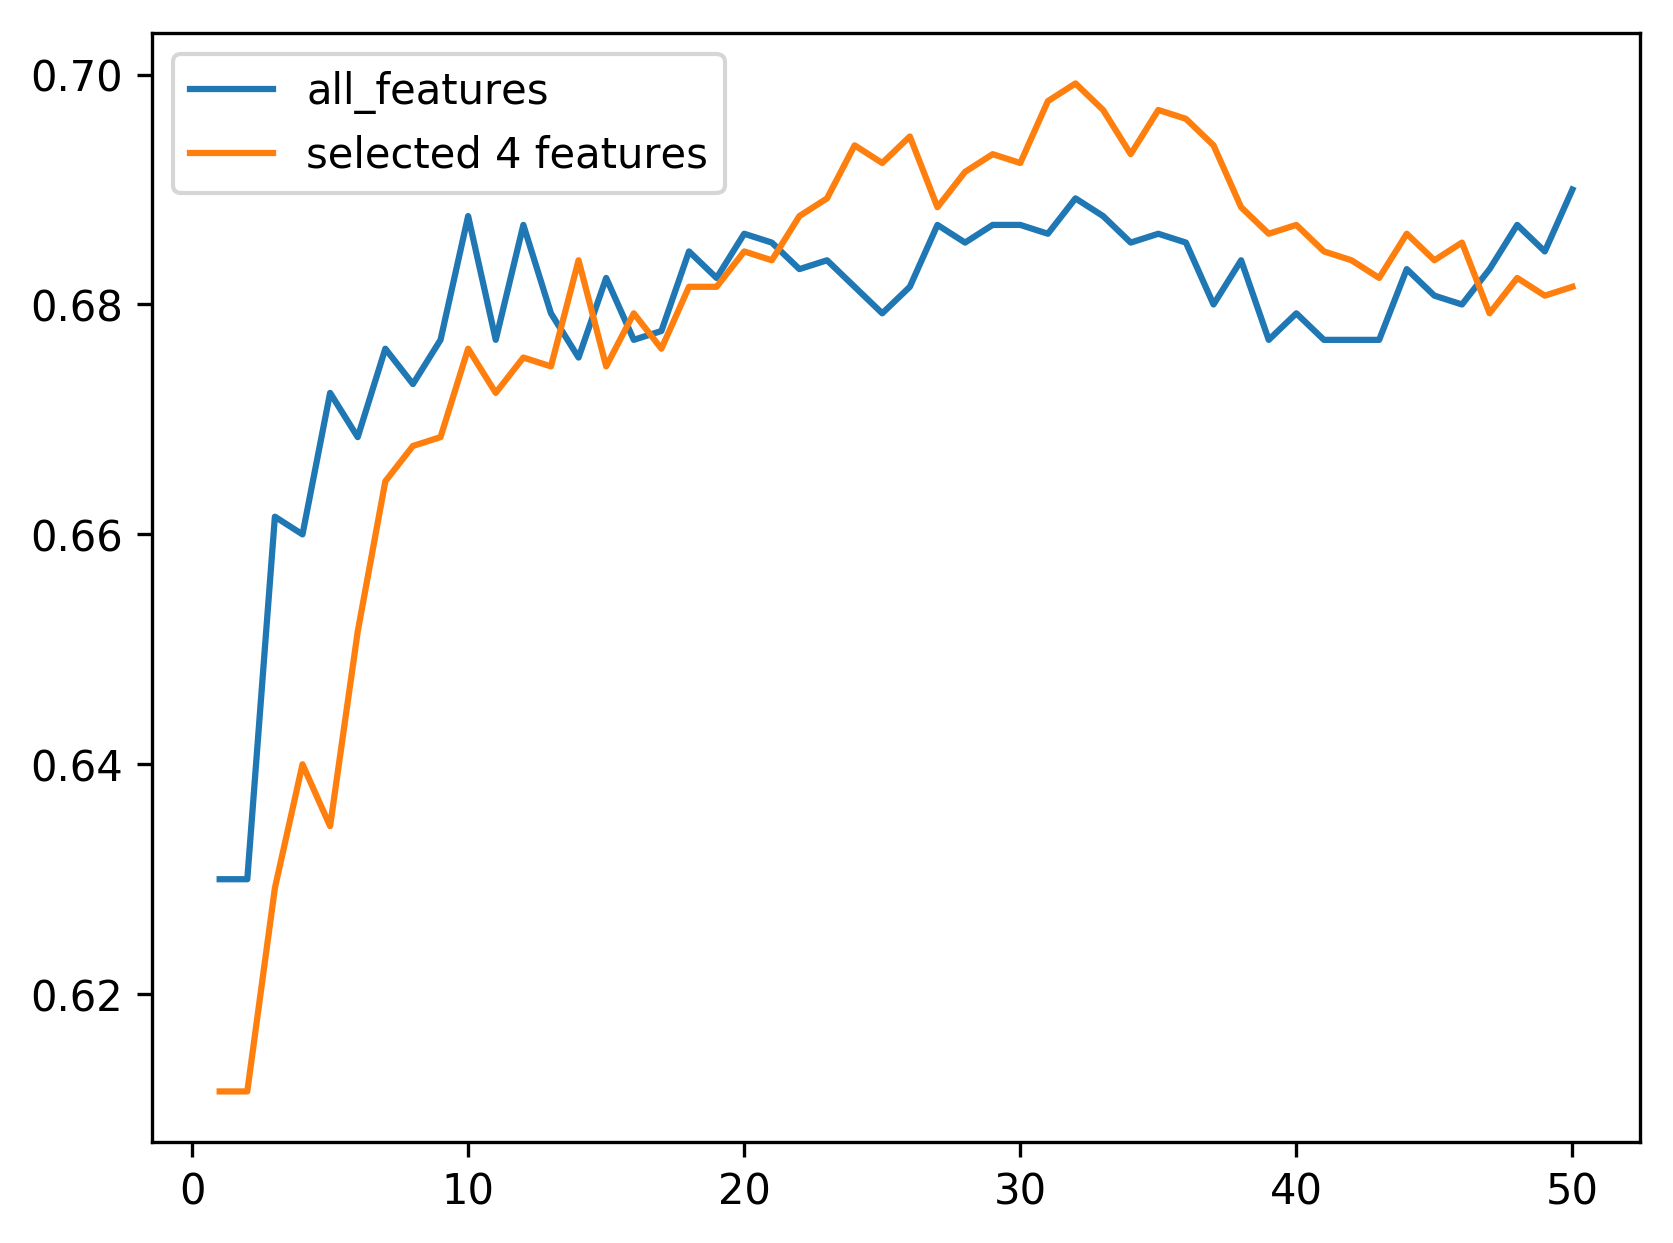
\includegraphics[width=9cm]{./select4features/quality_e.png}
\end{center}
\noindent
For quality prediction under uniform, using 'volatile acidity', 'total sulfur dioxide', 'density', 'alcohol' yields the best result.
\begin{center}
    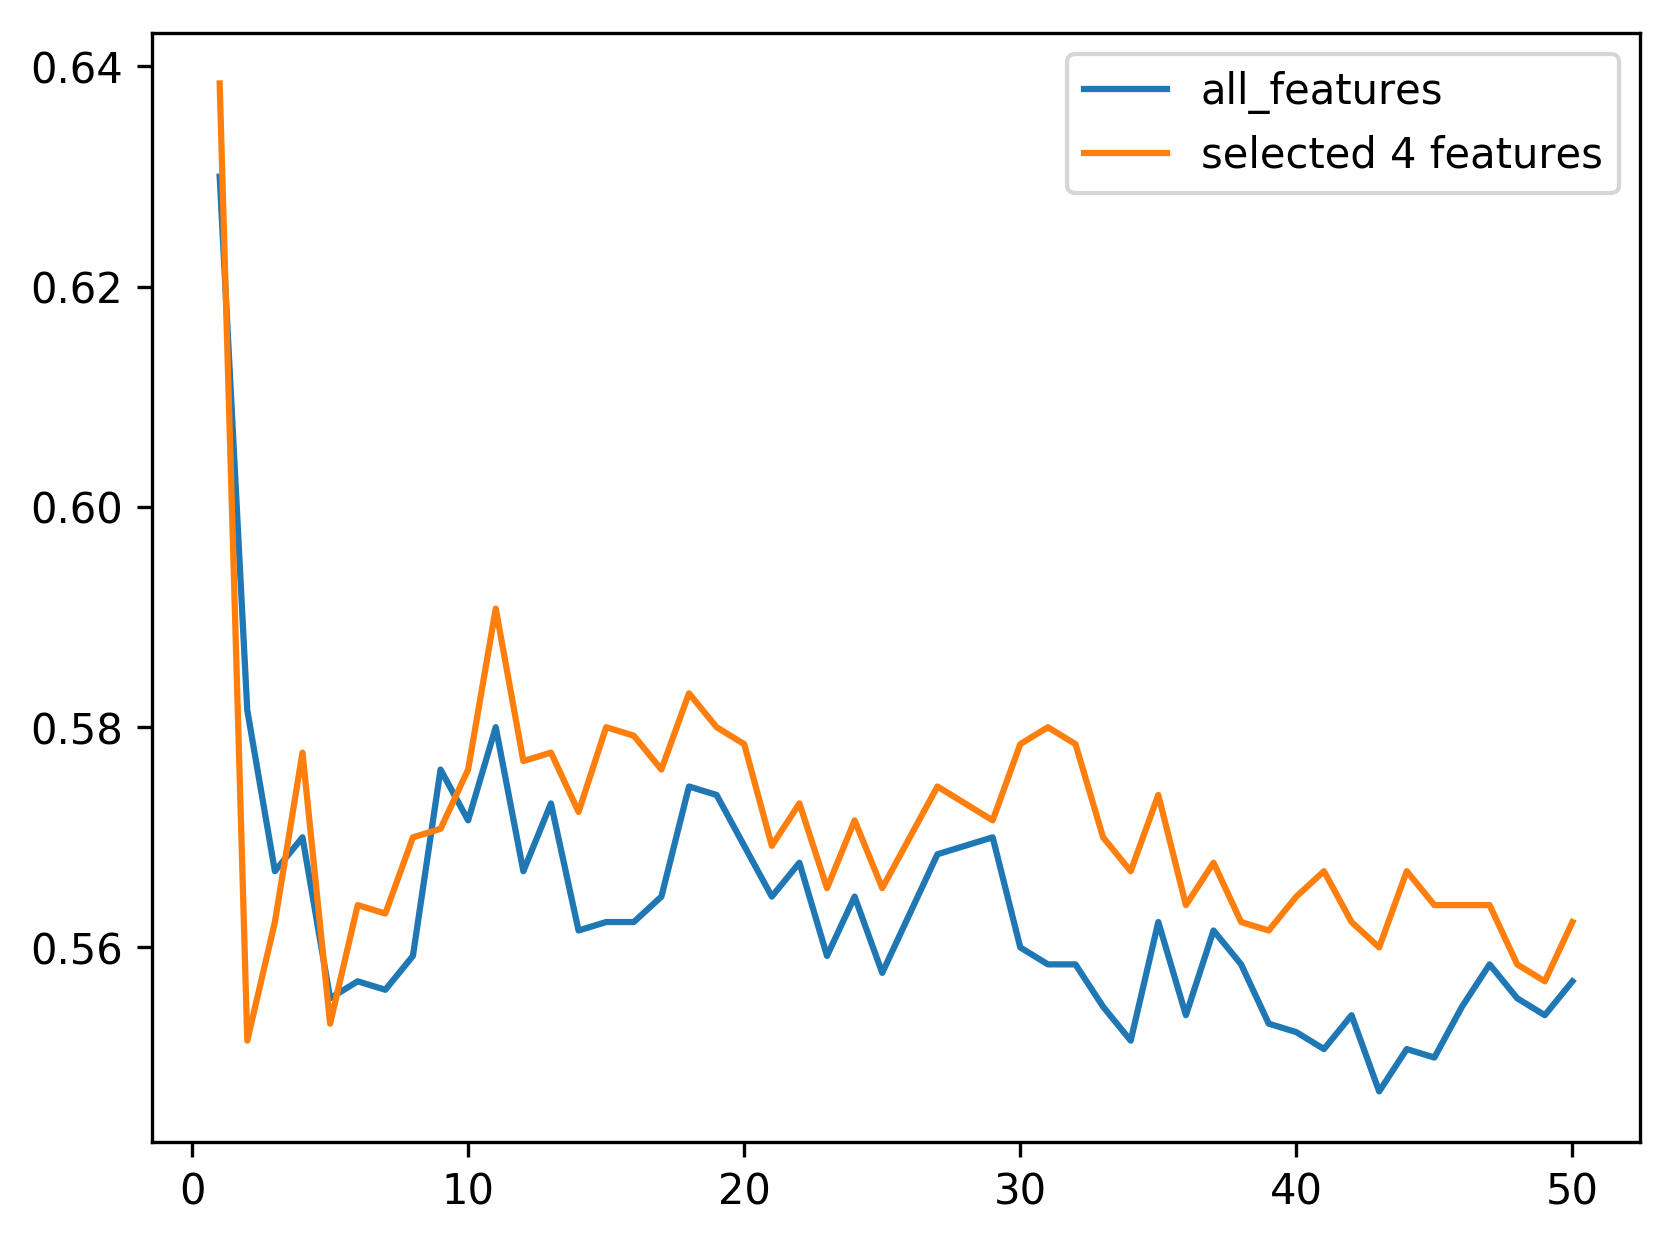
\includegraphics[width=9cm]{./select4features/quality_u.png}
\end{center}
\noindent
For color prediction, using euclidean+['residual sugar', 'total sulfur dioxide', 'density', 'alcohol'] has a better result than PCA and LDA.\\
For quality prediction, using euclidean+['volatile acidity', 'total sulfur dioxide', 'sulphates', 'alcohol'] has a better result than PCA and LDA.\\
\textbf{KNN Classification With PCA Components}
\begin{figure}[H]
\captionsetup[subfigure]{labelformat=empty}
\centering
\subfloat[]{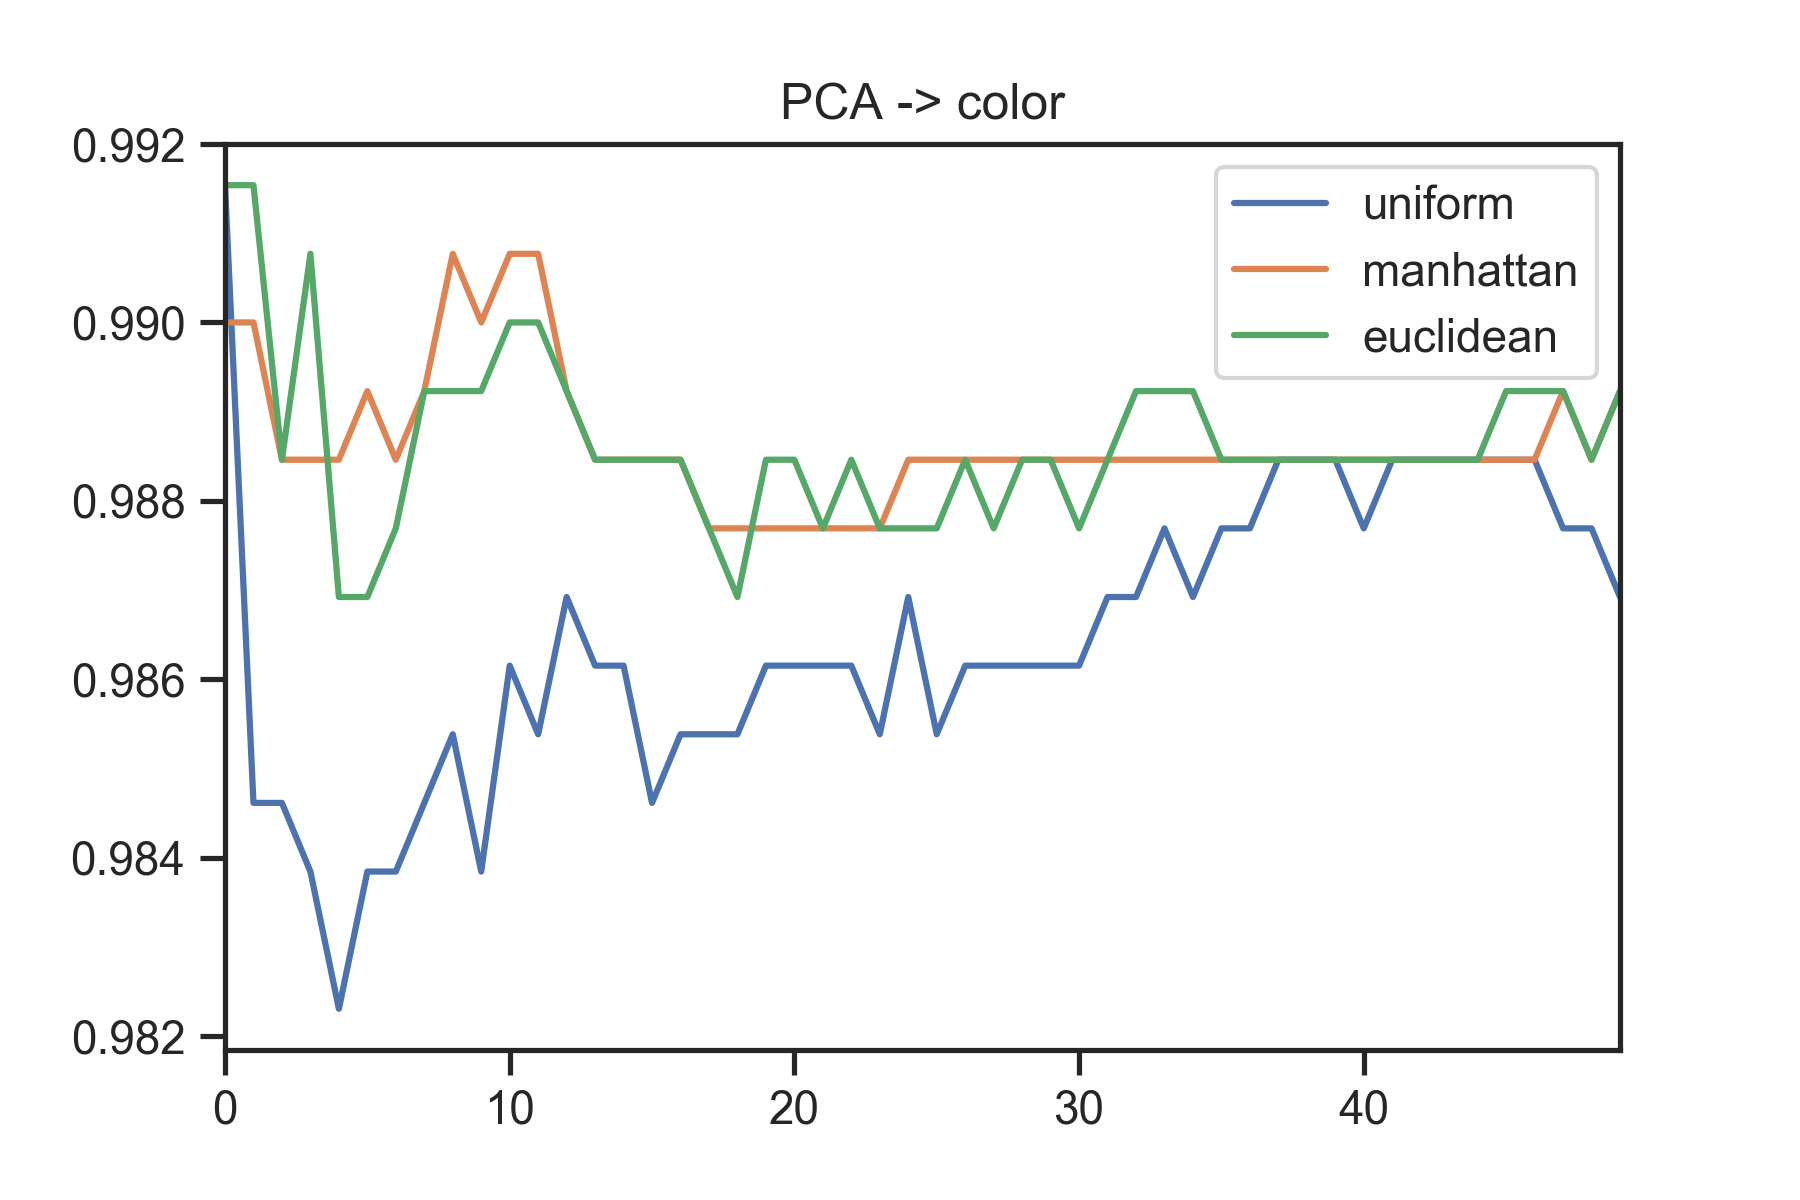
\includegraphics[width=0.48\textwidth]{Q1_PCA_color}}
\subfloat[] {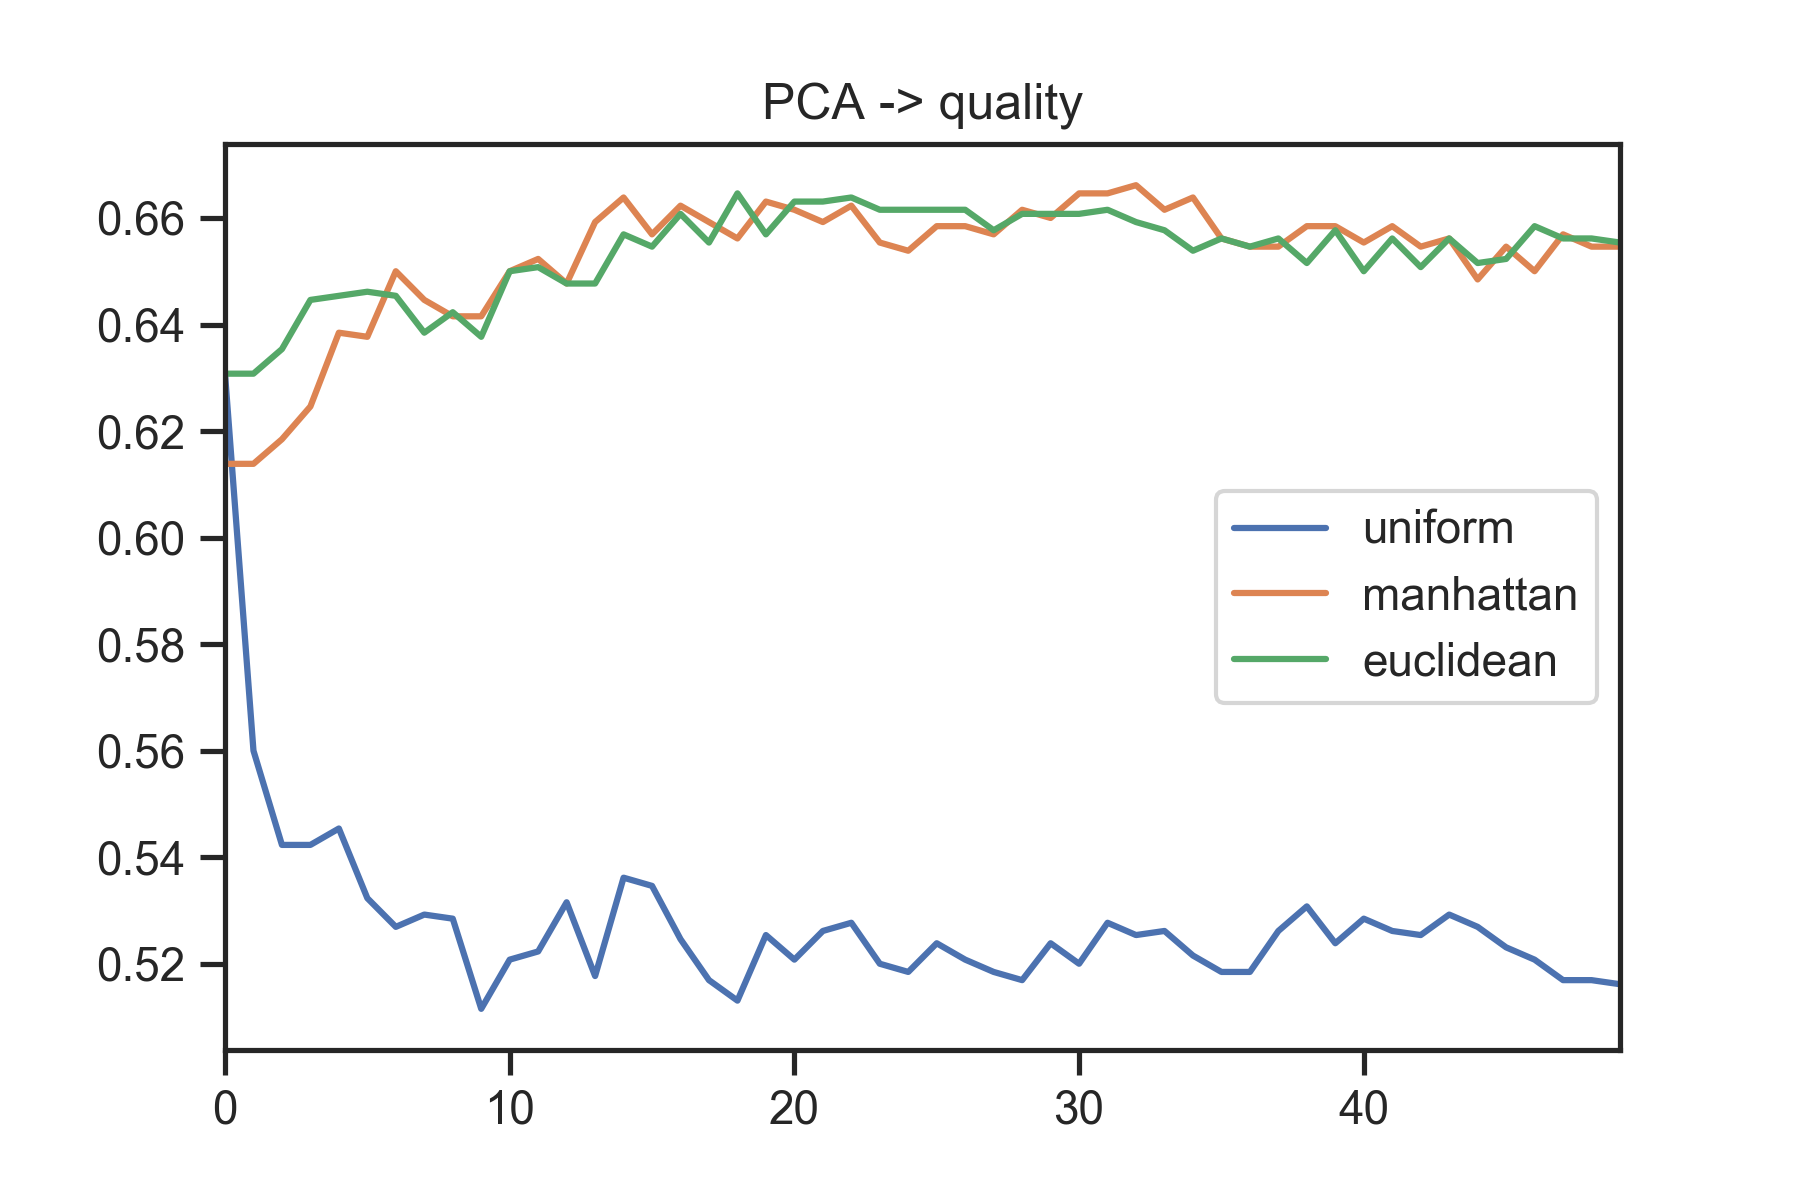
\includegraphics[width=0.48\textwidth]{Q1_PCA_quality.png}}
\end{figure}
\vspace*{-1.5cm}
\noindent
\textbf{KNN Classification With LDA Components}
\begin{figure}[H]
\captionsetup[subfigure]{labelformat=empty}
\centering
\subfloat[]{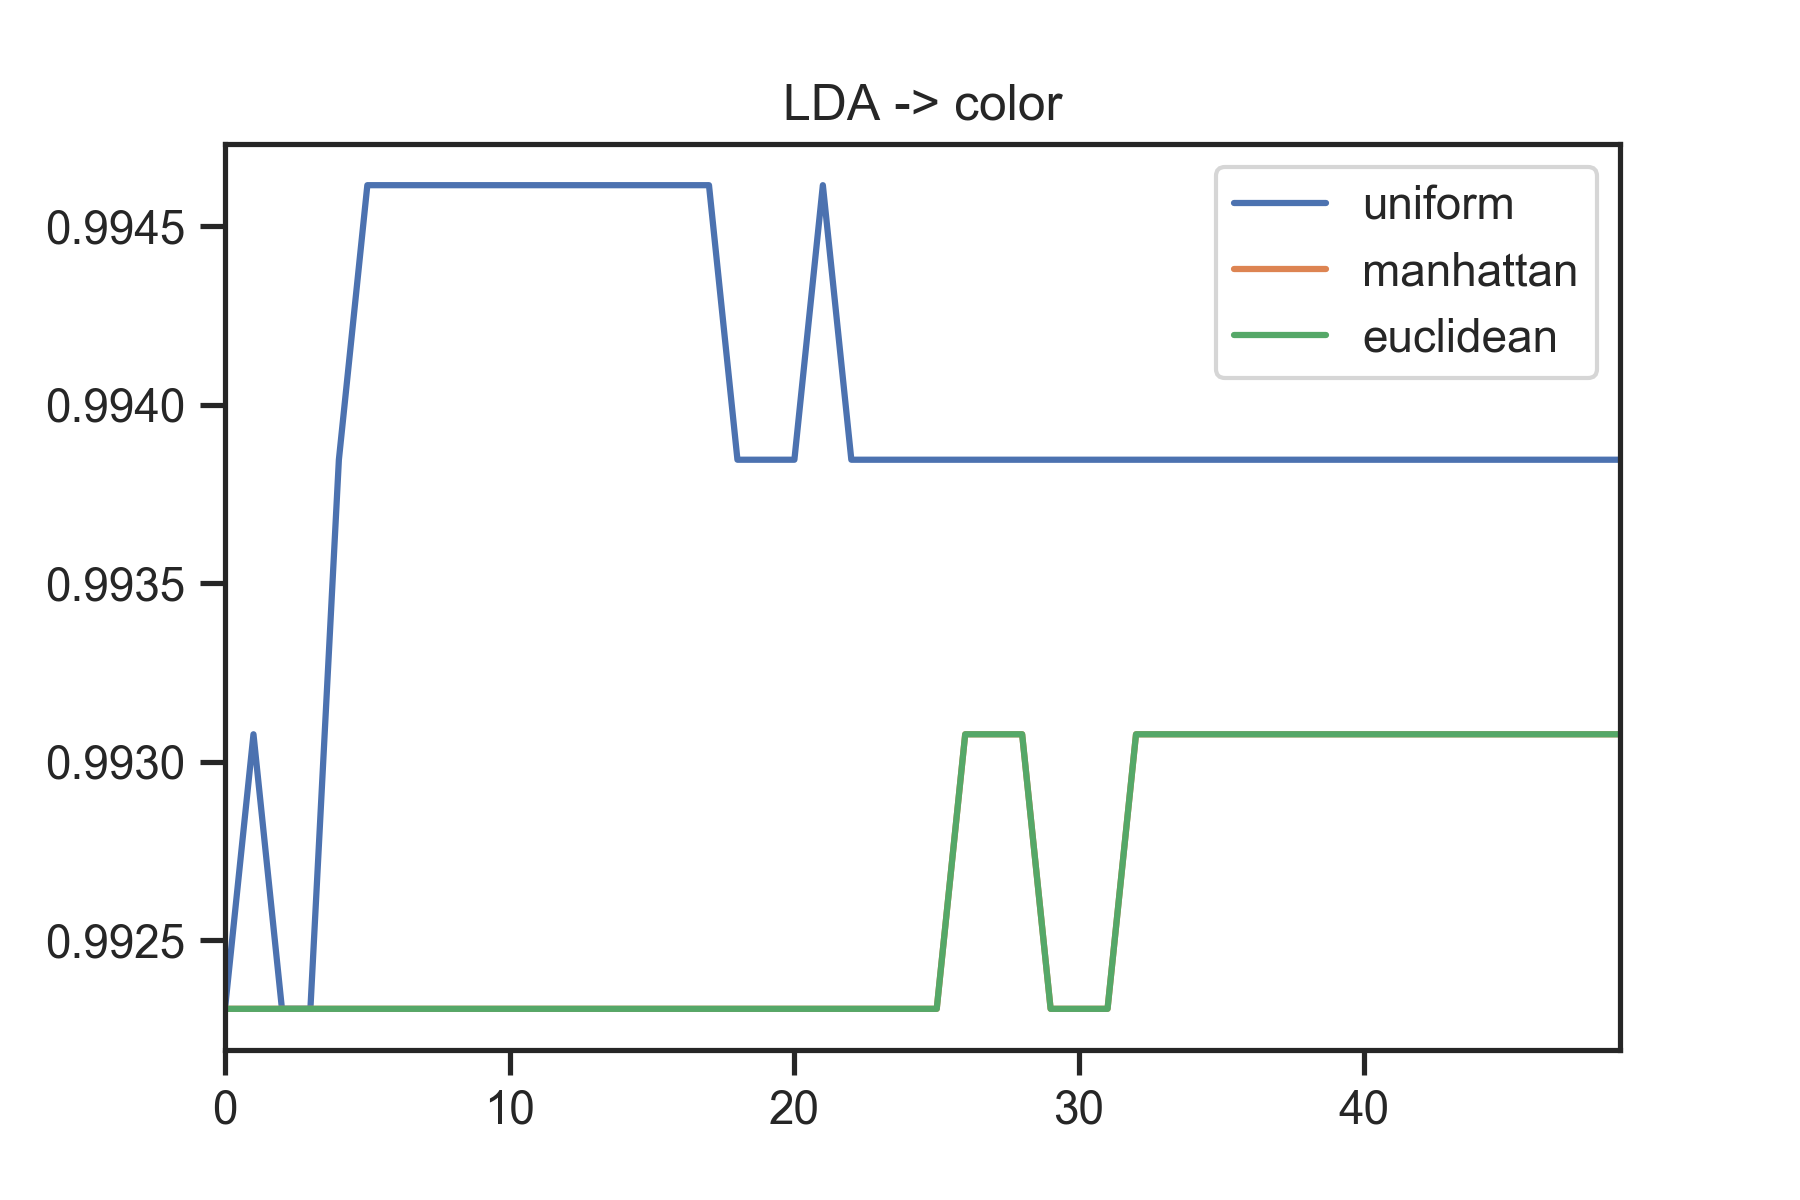
\includegraphics[width=0.48\textwidth]{Q1_LDA_color}}
\subfloat[] {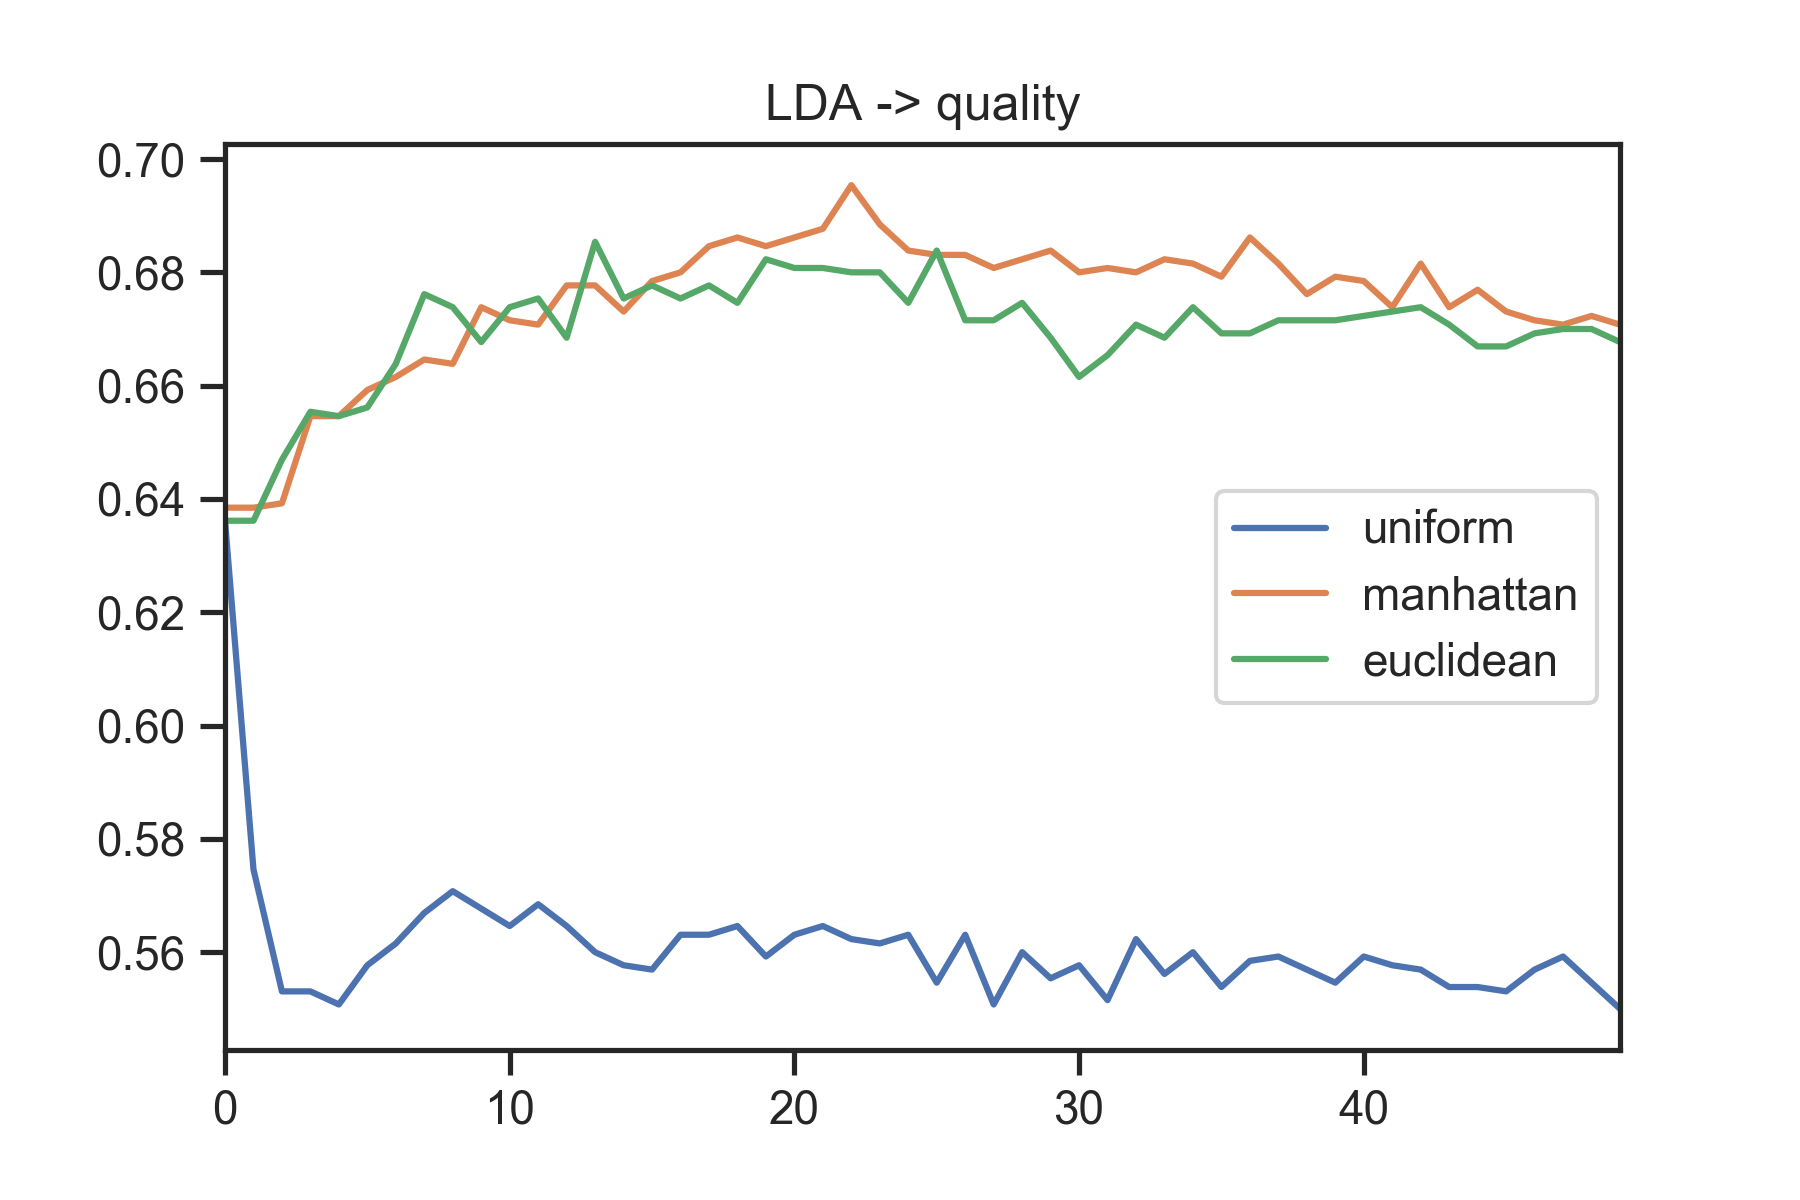
\includegraphics[width=0.48\textwidth]{Q1_LDA_quality.png}}
\end{figure}
\noindent
\textbf{Compare Performance Differences between PCA and LDA}\\
Generally, LDA performs slightly better than PCA. And using distance weight is better than using uniform weight except when using LDA to predict color, in which uniform weight is the best.
\end{document}